\section{دیتاست حملات سایبری دستگاه‌های اینترنت اشیا پزشکی \lr{CICIoMT2024}}

مهم‌ترین انگیزه برای توسعه این پژوهش \cite{dadkhah2024ciciomt2024} وجود کمبود در
داده‌های موجود ارزیابی کارایی تجهیزات اینترنت اشیا پزشکی و پیشرفت امنیتی تمام
شبکه‌هایی که در خصوص جریان‌های داده‌ای و پردازش داده‌های پزشکی کار می‌کنند،
می‌باشد بخصوص برای دستگاه‌های اینترنت اشیا پزشکی به دلیل اطلاعات حیاتی‌ای که
می‌توان به واسطه آن‌ها از بیماران با بیماری‌های مختلف مانیتور و دریافت کرد.
نتیجه این پژوهش دیتاستی از تمامی حملاتی مهم می‌باشد که روی دستگاه‌های \lr{IoMT}
انجام داده‌اند تا از طریق دیتاست بدست آمده بتوان به صورت خودکار با استفاده از
مدل‌های یادگیری ماشین وجود هر گونه حمله در سیستم‌های \lr{IoMT} را تشخیص داد و از
بروز آن جلوگیری کرد.

\subsection{اهداف اصلی پژوهش}

\begin{enumerate}
    \item کمک به پژوهشگران برای ایجاد سیستم‌های بهداشت و درمان ایمن با استفاده
    از سیستم‌های خودکار یادگیری ماشین و یادگیری عمیق.
    \item ارائه بنجمارک‌های واقعی برای ارزیابی و توسعه راهکار‌های امنیتی
    \item فراتر از شبیه‌سازی حملات، محققان تمام فرایند‌ها و چرخه حیات دستگاه‌های
    \lr{IoMT} را از ورود به شبکه تا خروج از طریق پروفایل‌های امنیتی رصد می‌کنند
    و به سیستم‌های خودکار مانند سیستم‌های طبقه‌بندی کننده حملات، اجازه می‌دهد تا
    ناهنجاری‌های امنیتی داخل سیستم‌های بهداشت و درمان را شناسایی کنند.
    \item با دیتاست بدست آمده \cite{ciciomt2024Dataset} که به صورت آزاد در دسترس
    عموم می‌باشد محققان راه‌های هوشمندانه‌ای را برای طبقه‌بندی حملات سایبری
    فراهم کرده‌اند.
\end{enumerate}

\subsection{پروتکل‌های استفاده شده}

برای حملات سایبری، محققان از پروتکل‌های پر استفاده در حوزه \lr{IoT} استفاده
کرده‌اند که عبارت‌اند از:

\begin{enumerate}
    \item \lr{Wi-Fi}
    \item \lr{MQTT}
    \item \lr{Bluetooth}
\end{enumerate}

این پژوهش در دسته‌بندی \lr{Predictive models} برای جلوگیری از حملات و حتی
فالت‌های نرم‌افزار می‌تواند قرار گیرد.

\subsection{دسته‌بندی حملات سایبری}

در این پژوهش ۱۸ حمله سایبری متفاوت روی ۴۰ دستگاه \lr{IoMT} صورت گرفته تا هم
بتوانند داده‌های مربوط به حملات را به صورت منظم و مهندسی شده فراهم کنند و هم
عملکرد دستگاه‌های \lr{IoMT} مورد نظر را با حملات سایبری مورد ارزیابی قرار دهند.

دسته‌بندی حملات:

\begin{LTR}
    \begin{itemize}
        \item DoS (Denial of Service)
        \item DDoS (Distributed Denial of Service)
        \item Spoofing
        \item Recon (Reconnaissance)
        \item MQTT (Message Queuing Telemetry Transport) attacks
    \end{itemize}
\end{LTR}

این ۱۸ حمله عبارت‌اند از:

\begin{LTR}
    \begin{itemize}
       \item DoS TCP
       \item DoS ICMP
       \item DoS SYN
       \item DoS UDP
       \item DDoS TCP
       \item DDoS ICMP
       \item DDoS SYN
       \item DDoS UDP
       \item MQTT Malformed Data
       \item MQTT DoS Connect flood
       \item MQTT DoS Publish flood
       \item MQTT DDoS Connect flood
       \item MQTT DDoS Publish flood
       \item ARP Spoofing (Man-in-the-Middle)
       \item Recon attacks
       \item Spoofing attacks
       \item Flooding campaigns (various types)
       \item Other targeted attacks specific to IoMT protocols
    \end{itemize}
\end{LTR}

\subsection{مقایسه \lr{CICIoMT2024} با کار‌های پیشین}

\subsubsection{دیتاست \lr{ECU-IoHT}}

این دیتاست \cite{ahmed2021ecu} آسیب‌پذیری دستگاه‌های \lr{IoT} را در محیط‌های
مراقبت‌های بهداشت و درمان بررسی کرده است. در این پژوهش دلیل اصلی حملات سایبری به
روز شدن تدابیر امنیتی دستگاه‌های واقعی بوده است که در حوزه مراقبت‌های بهداشتی و
درمانی توسعه یافته‌اند. این دستگاه از قبیل دستگاه‌های زیر بوده‌اند:

\begin{LTR}
    \begin{itemize}
        \item MySignals
        \item Temp sensor
        \item BP sensor
        \item HR sensor
        \item Bluettoth and wireless adapter
        \item Kali and windows laptop
    \end{itemize}
\end{LTR}

حملات سایبری انجام شده در این پرژوهش:

\begin{LTR}
    \begin{itemize}
        \item ARP spoofing
        \item DoS
        \item Smart and injection
    \end{itemize}
\end{LTR}

\subsubsection{حملات مخصوص روی فناوری بلوتوث}

در مطالعه دیگر \cite{zubair2022secure,skhs-0b39-21} دیتاستی فراهم شده است که
نشان می‌دهد حملات سایبری روی دستگاه‌های \lr{IoMT} در توپولوژی بلوتوث به چه شکلی
انجام می‌شوند. در این پژوهش بحث‌های تخصصی زیادی در رابطه با جنبه‌های استفاده از
این پروتکل شده است به گونه‌ای که اتصال چندین دستگاه به یک منبع، و حملات مختلفی
را روی این فناوری اجرا کرده‌اند. خروجی این حملات به گونه‌ای بوده است که می‌توان
عملکرد دستگاه‌ها را با استفاده از الگوریتم‌های یادگیری ماشین مانند \lr{SVM
(Support Vector Machine)}، \lr{K-Means} و شبکه‌های عصبی عمیق ارزیابی کرد.

\subsubsection{شبیه‌سازی ترافیک با ابزار \lr{IoTFlock،}}

در پژوهش دیگر \cite{hussain2021framework} محققان با استفاده از \lr{IoTFlock}،
ابزاری برای شبیه‌سازی ترافیک شبکه‌ای در سیستم‌های \lr{IoT} و شناسایی نقاط ضعف
امنیتی، به‌ویژه در حوزه سلامت، ارائه کرده‌اند.  این ابزار به پژوهشگران کمک
می‌کند تا راه‌حل‌های امنیتی قوی‌تری برای مقابله با حملات سایبری توسعه دهند.
ابزار \lr{IoTFlock} شبیه‌سازی ترافیک عادی شبکه و ترافیک مخرب را انجام می‌دهد.
حملاتی که در این پژوهش انجام شده‌اند عبارت‌اند از:

\begin{LTR}
    \begin{itemize}
        \item DDoS
        \item Brute force
        \item SlowITE
        \item MQTT Publish Flood
    \end{itemize}
\end{LTR}

حمله \lr{SlowITE} حمله هوشمندانه‌ای است که منابع سیستم را به آرامی خالی می‌کند
به گونه‌ای که هیچ چیز مشکوک به نظر نرسید.

\subsection{فرایند‌ها}

\subsubsection{آزمایشگاه \lr{IoT}}

برای انجام این پژوهش، محققان به دنبال یک آزمایشگاه مجهز به دستگاه‌های \lr{IoT}
بودند تا بتوانند آزمایش‌های مورد نظر را بر روی طیف عظیمی از دستگاه‌های پر
استفاده انجام دهند. این امر برای محققان کمی دشوار بود زیرا تنها به دستگاه‌های
\lr{IoT} نیاز نداشتند بلکه وجود تجهیزاتی مانند روتر‌ها، اکسس‌پوینت‌ها، سویچ‌ها و
تیمی که بتوانند تجیهیزات تحت شبکه را پیکربندی و راه‌اندازی کنند، ضروری بود. مشکل
بعد علاوه‌بر تامین منابع، راه‌اندازی این دستگاه‌ها در مقیاس بزرگ و هزینه‌های
متغیر بود که نیازمند سرمایه‌گذاری بودند تا با وجود اهمیت پژوهش، تجهیزات مورد نظر
را تهیه و پشتیبانی کند. از این رو موسسه کانادایی امنیت سایبری یا \lr{CIC} به
صورت داوطلب درخواست محققان را پذیرفت و آزمایشگاه مورد نظر را برای انجام این
تحقیقات ایجاد کرد که شامل ده‌ها دستگاه \lr{IoT} برای اهداف متنوعی مانند مراقبت
از بهداشت، خانه هوشمند را به همراه سیستم‌های شبکه‌ای و کیت‌های \lr{Arduino} و
\lr{RPi} را در اختیار آن‌ها گذاشت. در پی تجهیزات یک تیم فنی متعهد به نگهداری و
مدیریت دستگاه‌های \lr{IoT} و تمام تجهیزات تحت شبکه را به این کار دعوت کردند تا
محققان درگیر راه‌اندازی‌ها و پیکربندی‌های شبکه نشوند.

\begin{figure}[H]
  \centering
  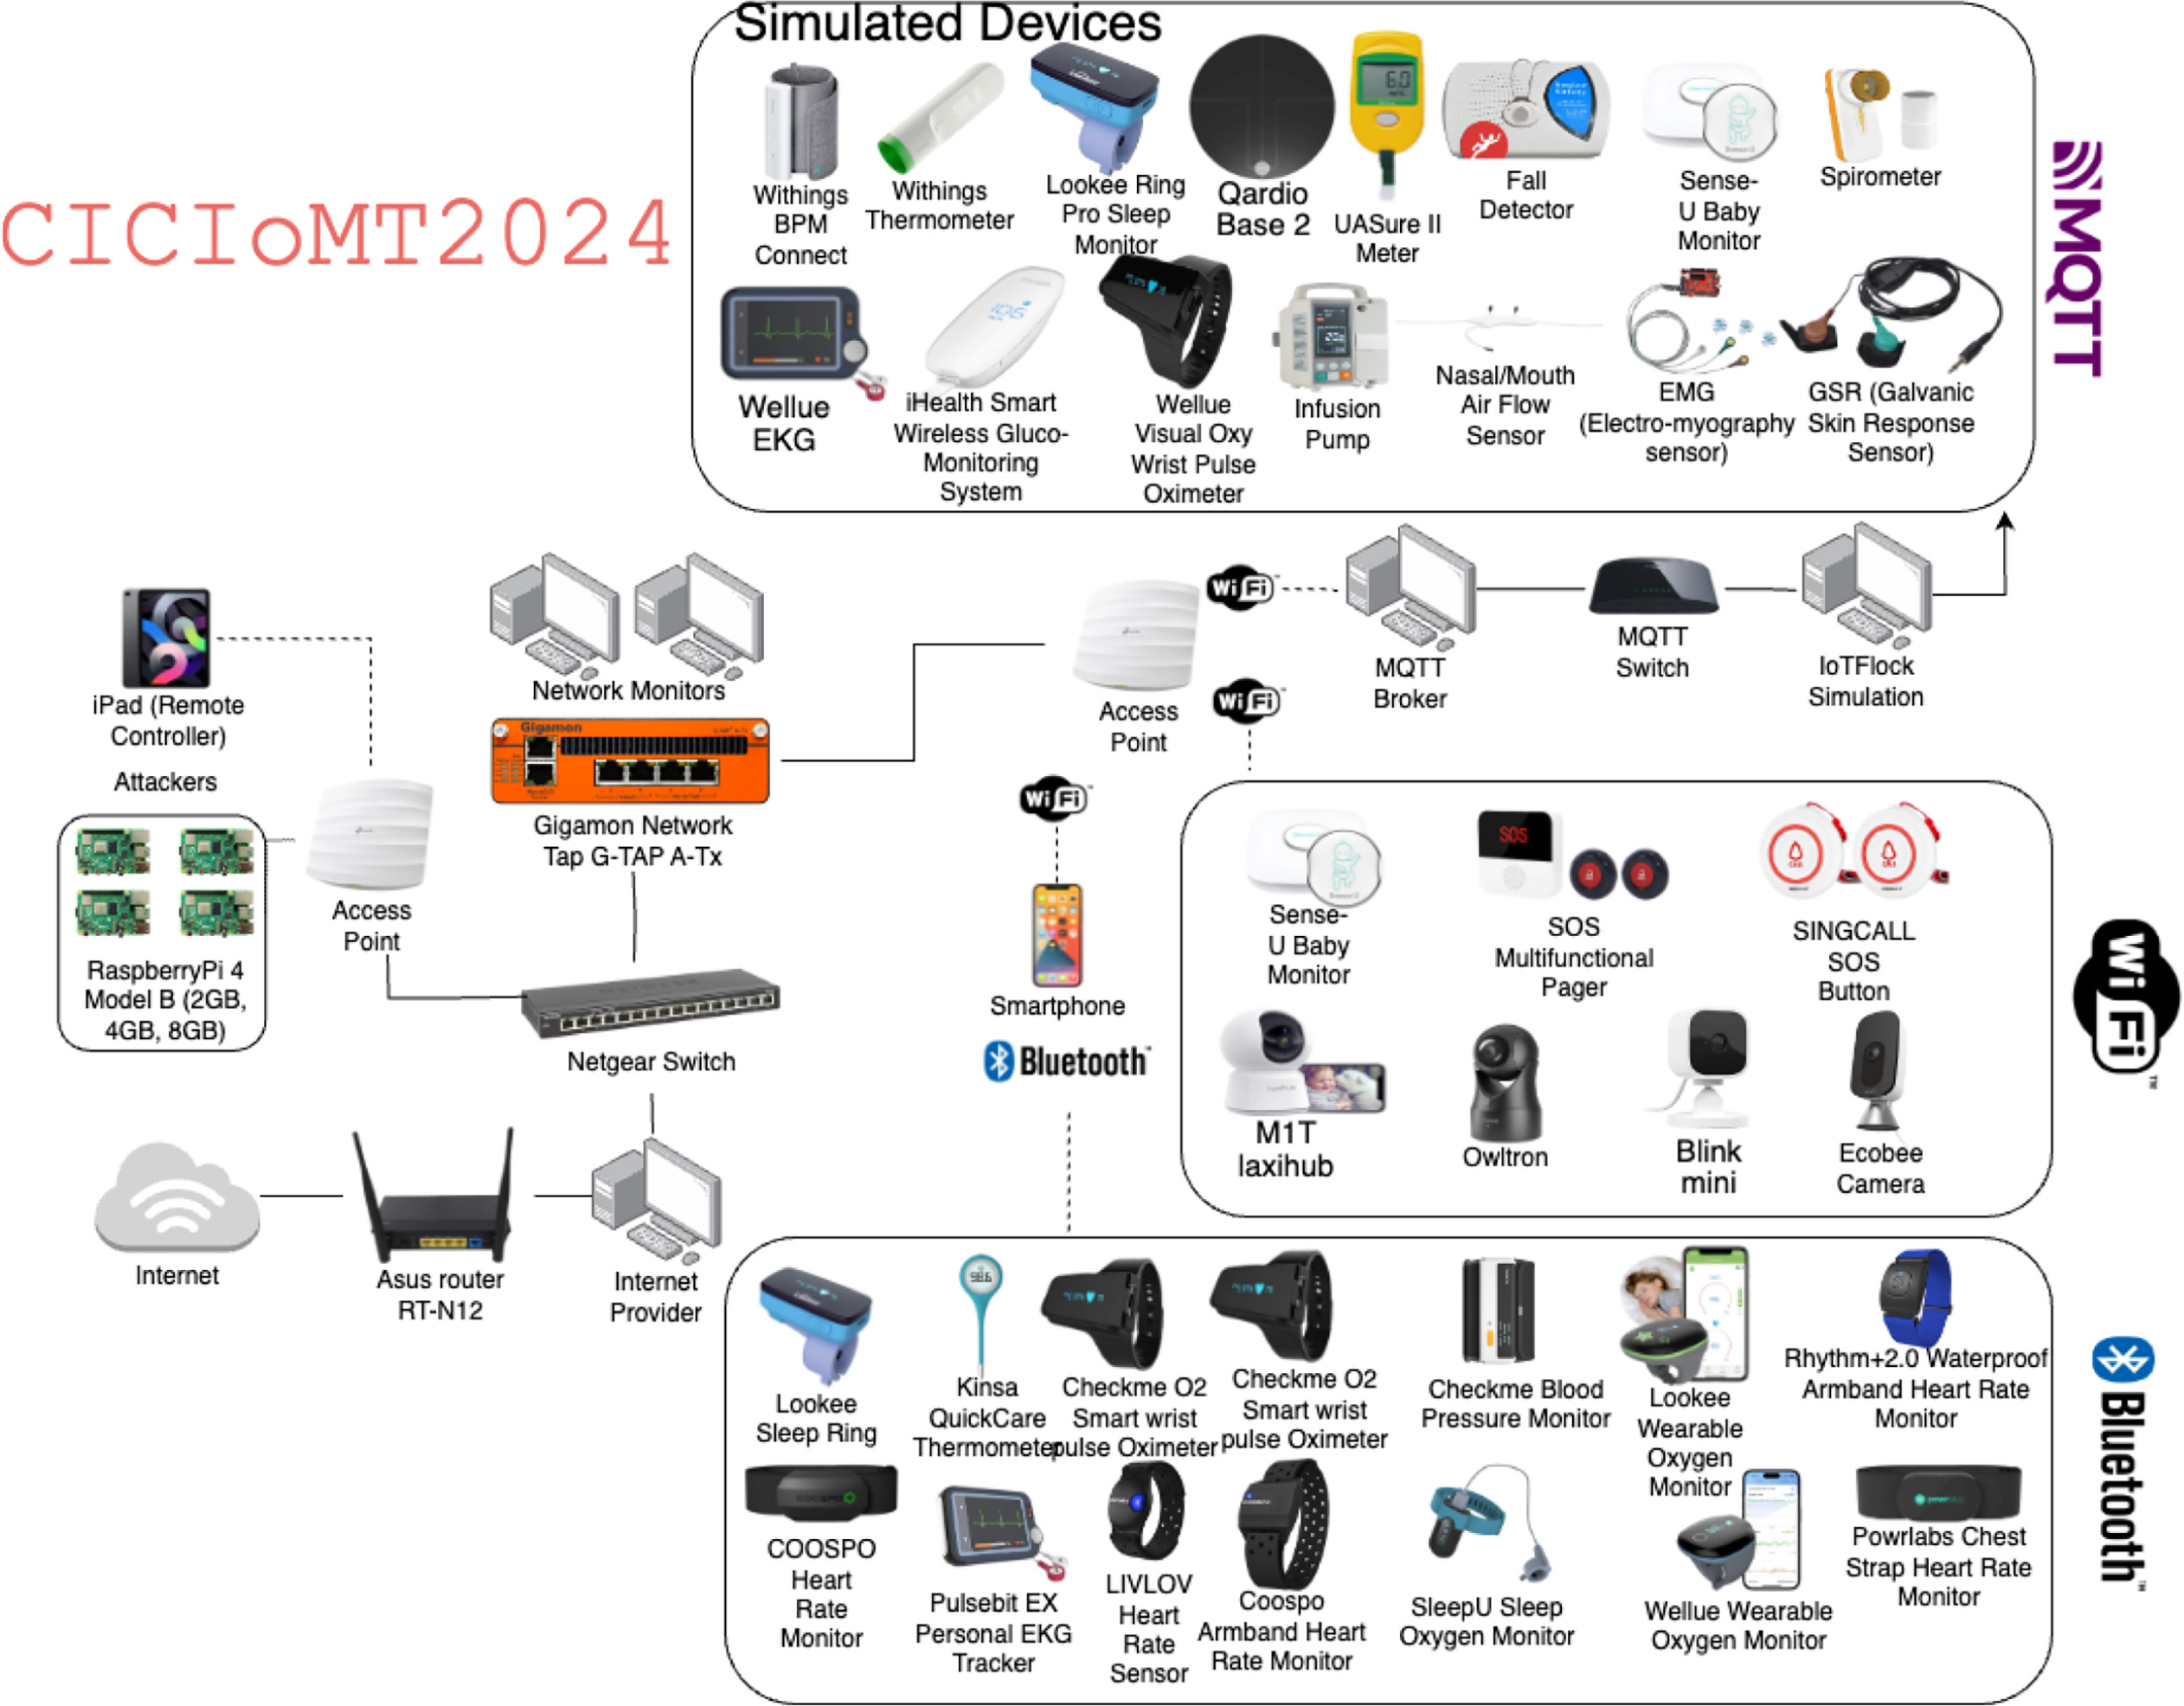
\includegraphics[width=0.7\textwidth]{./figures/fig-3.jpg}
  \caption{تجهیزاتی که موسسه کانادایی امنیت سایبری در اختیار محققان قرار داد.}
  \label{fig:cicIotLab}
\end{figure}

\subsubsection{توپولوژی شبکه دستگاه‌های \lr{IoMT}}

توپولوژی که محققان این پژوهش برای انجام آزمایشات خود راه‌اندازی کردند شامل
المان‌های زیر بوده است:

\begin{itemize}
    \item یک \lr{iPad} جهت کنترل فرایند‌ها و درخواست‌ها
    \item ۴ عدد \lr{RPi} که تمامی حملات از طریق آن‌ها انجام می‌شود.
    \item دستگاه‌های \lr{IoMT} که به وسیله یک \lr{Access point} به شبکه متصل
    هستند. با استفاده از این اتصال دستگاه‌های \lr{IoMT} می‌توانند به اینترنت
    دسترسی داشته باشند.
    \item تبادل داده‌ها بین دستگاه‌های \lr{IoMT} به گونه‌ای است که ۱۵، ۷ و ۱۴
    دستگاه به ترتیب با پروتکل‌های \lr{MQTT}، \lr{Wi-Fi} و بلوتوث ارتباط دارند.
\end{itemize}

\subsubsection{تولید ترافیک مخرب}

برای تولید ترافیک مخرب روی دستگاه‌های \lr{IoMT} از سناریو‌های واقعی در محیط‌های
مراقبت‌های بهداشتی استفاده شده است تا دیتاست کاملاً واقعی باشد. هدف این فرایند
ثبت ویژگی‌های ترافیک بدخیم و خراب‌کننده جهت تسهیل توسعه راهکار‌های امنیت سایبری
برای محیط‌های \lr{IoMT} می‌باشد. حملاتی که در این مرحله انجام شده عبارت‌اند از:

\begin{LTR}
    \begin{itemize}
        \item DoS
        \item DDoS
        \item ARP Spoofing
        \item Flooding campaings (Wi-Fi devices)
        \begin{itemize}
            \item ICMP
            \item SYN
            \item TCP
            \item UDP
        \end{itemize}
    \end{itemize}
\end{LTR}

\subsubsection{\lr{Wi-Fi}}

برای ایجاد ترافیک در این پروتکل ارتباطی، محققان حملات \lr{ARP Spoofing} را برای
\lr{Man in the middle} و بسیاری از حملات، \lr{TCP}، \lr{CYN}، \lr{ICMP} و
\lr{UDP} انجام دادند که همگی در دسته‌بندی \lr{DoS} و \lr{DDoS} قرار دارند.

\subsubsection{\lr{MQTT}}

در طی فعالیت‌ها در این پروتکل سه حمله انجام شده است:

\begin{itemize}
    \item \lr{MQTT Connect Flood}: در این حمله درخواست اتصال به \lr{Broker} با
    شدت زیاد ارسال می‌شود.
    \item \lr{MQTT Publish Flood}: ارسال بسته‌های مختلف به \lr{Topic}های مختلف و
    رندوم را انجام می‌دهد.
    \item \lr{MQTT Malformed Data Attack}: ارسال داده‌های نادرست را به
    \lr{Broker} برای تجزیه و تحلیل رفتار و جمع‌آوری اطلاعات \lr{Topic}های
    استفاده می‌کند.
\end{itemize}

در حمله آخر از ابزار \lr{MQTTSA} استفاده شد و سعی در \lr{Sniff} و شنود
\lr{Broker} با ارسال بسته‌های مشخص را داشتند تا رفتار دستگاه‌ها را بررسی کنند.
در این فرایند حمله، حمله‌کننده نام تمام تاپیک‌های \lr{MQTT} را که به صورت نهایی
منتشر شده‌اند را بدست می‌آورد و سعی می‌کند که به هر تاپیک داده نادرست را ارسال
کند. هدف اصلی این حملات بررسی و ارزیابی آسیب‌پذیری دستگاه‌های \lr{IoMT} در
پروتکل \lr{MQTT} بود. شبیه‌ساز با استفاده از ماشین مجازی \lr{VMware} که سیستم
عامل لینوکس اوبونتو نسخه $18.04.6$ راه‌اندازی شده بود و از نسخه \lr{GUI}
\lr{IoTFlock} که با زبان \lr{C++} نوشته شده بود مورد استفاده قرار گرفت.

\subsubsection{\lr{Bluetooth BLE 5.0}}

به طور کلی این ارزیابی برای بررسی مقاومت و تاب‌آوری دستگاه‌ها در برابر تهدیدات
امنیتی و اختلالات محیطی انجام شده است.

معمولاً حمله در بستر \lr{BLE} دو شرط الزامی را به همراه دارد:

\begin{enumerate}
    \item اجرای حمله
    \item جمع‌آوری ترافیک شبکه به روش‌ها و تکنیک‌های خاص
\end{enumerate}

فناوری \lr{BLE} به دلیل طراحی خاص خود که برای مصرف پایین انرژی بهینه شده است،
رفتاری متفاوت از پروتکل‌های بی‌سیم یا شبکه‌های معمولی دارد. بنابراین، اجرای
حملات یا ضبط ترافیک در این فناوری نیازمند ابزارها و تکنیک‌های متفاوتی است
\cite{matHackingTheBLE}. در این پژوهش، برای اجرای این حملات از یک تلفن همراه
هوشمند که به دستگاه \lr{BLE} متصل شده، استفاده شده است و سپس فعالیت‌های مخرب با
استفاده از کامپیوتر صورت گرفته است.

برای توسعه برنامه‌ای که قادر باشد تمامی بلوتوث‌های موجود در شبکه را جست‌وجو کند،
از کتابخانه \lr{Bleak} در زبان پایتون استفاده شده است. این برنامه توسعه‌یافته
می‌تواند به دستگاه‌های \lr{IoMT} متصل شده و تمامی سرویس‌ها و مشخصات آن‌ها را
دریافت کند. مشخصات دستگاه‌های \lr{IoMT} این امکان را فراهم می‌کند که دستگاه را
به شیوه‌ای خاص از عملکرد صحیح خود خارج کرد.

در ابتدا، برنامه بسته‌هایی با طول‌های مختلف ارسال می‌کند. طول هر بسته بین ۲۰ تا
۸۱۰ بایت، با افزایش ۱۰ بایتی تنظیم شده است. داده‌های ارسالی به شکل الگوی تکراری
مانند $01234567890123456\ldots$ هستند که اعداد به صورت پشت سر هم تکرار می‌شوند.
هر بار که ارسال موفقیت‌آمیز انجام می‌شود، لاگ مربوطه ثبت می‌گردد. سپس برنامه
مشخص می‌کند که هر بسته با موفقیت روی کدام \lr{UUID} ارسال شده است.

آدرس \lr{UUID} که مشابه \lr{SSID} در شبکه‌های بی‌سیم \lr{Wi-Fi} است، برای مشخص
کردن آدرس شبکه بلوتوث استفاده می‌شود. پس از این مرحله، برنامه وارد حلقه‌ای
می‌شود که داده‌ها روی \lr{UUID}های شناسایی‌شده ارسال می‌شوند و در نهایت در یک
متغیر ذخیره می‌گردند. این ارسال‌های پی‌درپی به منظور ایجاد بار اضافی
(\lr{Overload}) در دستگاه انجام می‌شوند که منجر به اختلال در عملکرد صحیح دستگاه
شده و حمله‌ای شبیه به \lr{DoS} را شبیه‌سازی می‌کند.

داده‌ها به دو روش جمع‌آوری می‌شوند. در روش اول، لاگ‌های سمت دستگاه اندروید که به
دستگاه \lr{IoT} متصل است، بررسی می‌شوند. روش دوم شامل استفاده از \lr{Sniff} شبکه
بلوتوث با استفاده از برد \lr{Ubertooth} است که از طریق کامپیوتر متصل شده و
قابلیت شناسایی تمامی بلوتوث‌های موجود در محدوده را فراهم می‌کند.

هدف اصلی از تحلیل این دو نوع لاگ، دستیابی به یک درک جامع و کلان از رفتار
دستگاه‌ها در حالت عادی و هنگام وقوع حمله است. این حملات به شکل‌های مختلف آنقدر
تکرار می‌شود تا نتیجه‌اش را به عنوان بررسی انعطاف‌پذیری و آسیب‌پذیری دستگاه در
بستر حمله‌های مبتنی بر \lr{BLE} ثبت کنند.

دستگاه‌های \lr{IoMT} که در این حمله شرکت داشته‌اند به صورت زیر می‌باشد که هر
کدام رفتار متفاوتی را نسبت به حملات داشته‌اند:

\begin{table}[h!]
    \centering
    \begin{tabular}{|l|p{10cm}|}
        \hline
        \textbf{نام دستگاه} & \textbf{نتیجه بررسی} \\ \hline
        \lr{Lookee Sleep Ring} & بدون وقفه عملکرد دستگاه در طی حملات مورد تأیید قرار گرفت. \\ \hline
        \lr{Powerlabs HR Monitor Arm Band} & دستگاه باید طبق استانداردها، حتی تحت حمله عملکرد صحیح خود را داشته باشد. \\ \hline
        \lr{COOSPO HW807 Armband} & حملات منجر به ایجاد اختلال و خاموش شدن دستگاه شدند که نشان‌دهنده شکست سخت‌افزار در برابر عوامل خارجی است. \\ \hline
        \lr{Livlov Heart Rate sensor} & سنسور بدون وقفه در برابر حملات مقاومت کرد. \\ \hline
        \lr{Wellue O2 Ring} & دستگاه بدون وقفه به عملیات خود ادامه داد. \\ \hline
        \lr{Lookee O2 Ring} & دستگاه تحت تأثیر حملات دچار اختلال شدید شد و خاموش شد. \\ \hline
        \lr{Checkme BP2A} & دستگاه داده‌ها را فقط در صورت اتصال پایدار بلوتوث ارسال می‌کرد، که نشان‌دهنده طراحی ایمن برای حفظ امنیت داده‌ها است. \\ \hline
        \lr{SleepU Sleep Oxygen Monitor} & در برابر حملات مقاومت کرده و بدون وقفه عمل کرده است. \\ \hline
        \lr{Rhythm+2.0 (Scosche)} & دستگاه به شدت تحت تأثیر حمله قرار گرفت و خاموش شد. \\ \hline
        \lr{Wellue Pulsebit EX} & دستگاه در برابر حملات مقاومت کرد و بدون قطعی به عملیات خود ادامه داد. \\ \hline
        \lr{Checkme O2 Smart Pulse Oximeter} & دستگاه مقاومت کرده و به عملیات استاندارد خود ادامه داده است. \\ \hline
        \lr{Kinsa Thermometer} & تحت تأثیر حملات قرار گرفت و تنها راه ریست کردن اتصال، تخلیه باتری بود. \\ \hline
        \end{tabular}
        \caption{نتایج بررسی دستگاه‌ها تحت حملات مختلف}
    \label{table:attack_results}
\end{table}

لازم به ذکر است که تمام حملات صورت گرفته کاملاً در محیطی ایزوله از هر گونه
سیگنال خارجی انجام شده است تا با ترافیک شبکه جمع‌آوری شده هیچ سیگنال مزاحمی
وجود نداشته باشد.

\subsection{\lr{IoMT profiling}}

درک کامل جنبه‌های مختلف رفتار عملیاتی دستگاه‌های \lr{IoMT} برای بهبود امنیت سیستم
بسیار حیاتی است. ارزیابی پروفایل‌های \lr{IoMT} قابلیت کلاسیفایرها را در تشخیص
ناهنجاری‌های عملکردی دستگاه‌های مراقبت بهداشتی تقویت کرده و امکان تمایز بین
رفتار عادی و غیرعادی شبکه را فراهم می‌سازد. در تسک‌هایی که کلاسیفای نشده‌اند،
الگوهای مشاهده‌نشده می‌توانند نشان‌دهنده فعالیت‌های مخرب و حملات zero-day باشند.

حملات \lr{zero-day} به نوعی حمله سایبری اشاره دارند که از یک آسیب‌پذیری ناشناخته
یا به‌تازگی کشف‌شده در نرم‌افزار، سخت‌افزار یا سیستم بهره می‌برند. نام این نوع
حمله از آنجا گرفته شده است که توسعه‌دهنده یا مالک سیستم پیش از وقوع حمله
برنامه‌ای برای شناسایی و رفع آسیب‌پذیری نداشته است. در این تحقیق، تمامی حملات
موردنظر شبیه‌سازی و بررسی شده‌اند تا توسعه‌دهندگان و شرکت‌ها بتوانند از قرار
گرفتن در معرض حملات \lr{zero-day} جلوگیری کنند.

ویژگی‌های اصلی حملات \lr{zero-day} \cite{enwiki:1268124149}:

\begin{itemize}
    \item آسیب‌پذیری ناشناخته: آسیب‌پذیری که هنوز توسط تیم امنیتی یا تیم توسعه
    کشف یا رفع نشده است.
    \item غالفگیری: به دلیل آگاهی از آسیب‌‌پذیری، سیستم‌ها در برابر این نوع
    حملات کامل آسیب‌پذیر هستند.
    \item سوء استفاده یا \lr{Exploit}: مهاجمان معمولاً از کد یا تکنیک‌هایی برای
    بهره‌برداری از آسیب‌پذیری استفاده می‌کنند.
\end{itemize}

\subsubsection{آزمایش‌های مبتنی بر انرژی و باتری}

آزمایش‌های این قسمت مربوط به مصرف انرژی دستگاه‌های مجهز به \lr{Wi-Fi} بوده است.
این آزمایش‌ها تلاش می‌کنند تا رفتار دستگاه‌های \lr{Wi-Fi} را از نظر مصرف انرژی و
ارسال داده‌ها در هنگام روشن و یا خاموش بودن را به دقت تحلیل کنند. این آزمایش
تنها روی هفت دستگاه \lr{Wi-Fi} تمرکز دارند و روی دستگاه‌های \lr{MQTT} شبیه‌سازی
نشده‌اند. برای انجام این آزمایش:

تمام دستگاه‌ها از شبکه خارج شده‌اند و به جایی متصل نخواهند بود. تنها دستگاه متصل
به شبکه یک دستگاه \lr{iPad} خواهد بود که برای کنترل و نظارت بر سایر دستگاه
استفاده می‌شود. حتی دستگاه‌های \lr{RPi} نیز در این آزمایش متصل نبودند. مراحل زیر
در ادامه انجام شده‌اند:

\begin{enumerate}
    \item در مرحله اول، دستگاه مورد نظر روشن شد و رفتار آن برای مدت ۲ دقیقه با
    استفاده از فیلتر آدرس \lr{MAC} ثبت شد.
    \item در مرحله دوم، دستگاه خاموش می‌شود و فرایند ثبت داده‌ها برای ۳ دقیقه
    دیگر ادامه پیدا می‌کند تا هر بسته اطلاعاتی باقی‌مانده شناسایی شوند و اطمینان
    حاصل شود که دیگر هیچ بسته‌ای ارسال نمی‌شود.
\end{enumerate}

فرایند انجام شده بالا دقیقاً همانند فرایندی است که در جمع‌آوری دیتاست
\lr{CICIoT2021} انجام شده بود. نکته قابل توجه آن است که برخی از دستگاه‌ها کلید
روشن و خاموش نداشتند و برای انجام آزمایش نیاز به انجام تنظیمات مخصوص داشتند:

\begin{LTR}
    \begin{itemize}
        \item Singcall Sensor
        \item SOS Multifunctional Page
        \item Sense U Baby
    \end{itemize}
\end{LTR}

\subsubsection{آزمایشگاه‌های مبتنی بر حالت \lr{Idle}}

آزمایشاتی است که تنها در زمان روشن بودن دستگاه ولی در حالی که هیچ داده‌ای منتقل
نمی‌کردن، انجام می‌شود. انجام این آزمایش به محققان اجازه داد که رفتار حالت عادی
و \lr{baseline} شبکه رو بهتر متوجه بشن. در این آزمایش ۱۳ ساعت عملیات بررسی و
آزمایش طول کشید. آزمایشات بین دو شب از ساعت ۶ عصر تا تا ۷ صبح برای اطمینان از
اینکه هیچ تعاملی دستگاه‌ها ندارند انجام شد.

\subsubsection{آزمایش‌های فعال}

شامل دستگاه‌هایی می‌شود که وظایف مورد نظر خود را انجام می‌دادند و ترافیک عادی را
در شبکه بابت عملیات خود ایجاد می‌کردند.

\subsubsection{آزمایش‌های مبتنی بر تعامل}

این قسمت از آزمایشات روی تعامل با دستگاه‌ها متمرکز است که به صورت زیر انجام
شده‌اند:

\begin{itemize}
    \item فیزیکی: کاربر مستقیماً با دستگاه ارتباط برقرار می‌کند.
    \item دیجیتالی:‌برنامه‌ها بایکدیگر ارتباط می‌گیرند و ارسال داده انجام
    می‌دهند.
\end{itemize}

سه نوع تعامل بررسی شده است:

\begin{itemize}
    \item تعامل فیزیکی:
    \begin{itemize}
        \item این آزمایشات زمانی انجام شده‌اند که دستگاه‌ها دارای دکمه فیزیکی
        بوده‌اند.
        \item آزمایشات با ترکیب تعامل فیزیکی و شبکه‌های محلی یا شبکه‌های گسترده
        صورت گرفته است:
        \begin{itemize}
            \item در شبکه محلی: اپلیکیشن و دستگاه در یک شبکه قرار دارند.
            \item در شبکه \lr{WAN}: اپلیکیشن از شبکه‌ای متفاوت نسبت به دستگاه
            متصل بوده است.
        \end{itemize}
    \end{itemize}
    \item تعامل در شبکه محلی:
    \begin{itemize}
        \item در این آزمایشات از اپلیکیشن‌های همراه دستگاه استفاده شده است.
        اپلیکیشن و دستگاه هر دو در یک شبکه با استفاده از \lr{Wi-Fi} بوده‌اند.
        برای مثال روشن و خاموش کردن دستگاه از طریق اپلیکیشن در خانه.
        \item در تعامل با شبکه گسترده نیز همینطور بوده است، اپلیکیشن همراه
        دستگاه به شبکه‌ای متفاوت متصل بوده و کنترل دستگاه از راه دور مثلاً روشن
        کردن دستگاه خانه از دفتر کار صورت گرفته است.
    \end{itemize}
\end{itemize}

\subsection{ارزیابی‌های مبتنی بر یادگیری ماشین}

آزمایشاتی که انجام شده آنقدر باعث تولید داده شد که می‌توان با استفاده از آن‌ها
ارزیابی‌هایی را برای تشخیص و جلوگیری حمله در سیستم‌های \lr{IoMT} انجام داد. از
جمله این مدل‌های یادگیری ماشین می‌توان به موارد زیر اشاره کرد:

\begin{LTR}
    \begin{itemize}
        \item Logistic Regression
        \item Random Forest
        \item Adaboost
        \item Deep Neural Networks (DNN)
    \end{itemize}
\end{LTR}

دسته‌بندی و طبقه‌بندی داده‌ها نیز می‌تواند به صورت \lr{attack} و \lr{Benign} یا
به صورت مشخص‌تر، \lr{Dos, MQTT, recon} و یا \lr{DDoS} انجام شود.